\documentclass{article}
\usepackage[utf8x]{inputenc}
\usepackage{ucs}
\usepackage{amsmath} 
\usepackage{amsfonts}
\usepackage{marvosym}
\usepackage{wasysym}
\usepackage{upgreek}
\usepackage[english,russian]{babel}
\usepackage{graphicx}
\usepackage{float}
\usepackage{textcomp}
\usepackage{hyperref}
\usepackage{geometry}
  \geometry{left=2cm}
  \geometry{right=1.5cm}
  \geometry{top=1cm}
  \geometry{bottom=2cm}
\usepackage{tikz}
\usepackage{ccaption}
\usepackage{multicol}

\hypersetup{
   colorlinks=true,
   citecolor=blue,
   linkcolor=black,
   urlcolor=blue
}

\usepackage{listings}
%\setlength{\columnsep}{1.5cm}
%\setlength{\columnseprule}{0.2pt}

\usepackage[absolute]{textpos}

\usepackage{colortbl,graphicx,tikz}
\definecolor{X}{rgb}{.5,.5,.5}

\renewcommand{\thesubsection}{\arabic{subsection}}

\begin{document}
\pagenumbering{gobble}
\lstset{
  language=C,                % choose the language of the code
  basicstyle=\linespread{1.1}\ttfamily,
  columns=fixed,
  fontadjust=true,
  basewidth=0.5em,
  keywordstyle=\color{blue}\bfseries,
  commentstyle=\color{gray},
  stringstyle=\ttfamily\color{orange!50!black},
  showstringspaces=false,
  numbersep=5pt,
  numberstyle=\tiny\color{black},
  numberfirstline=true,
  stepnumber=1,                   % the step between two line-numbers.        
  numbersep=10pt,                  % how far the line-numbers are from the code
  backgroundcolor=\color{white},  % choose the background color. You must add \usepackage{color}
  showstringspaces=false,         % underline spaces within strings
  captionpos=b,                   % sets the caption-position to bottom
  breaklines=true,                % sets automatic line breaking
  breakatwhitespace=true,         % sets if automatic breaks should only happen at whitespace
  xleftmargin=.2in,
  extendedchars=\true,
  keepspaces = true,
}
\lstset{literate=%
   *{0}{{{\color{red!20!violet}0}}}1
    {1}{{{\color{red!20!violet}1}}}1
    {2}{{{\color{red!20!violet}2}}}1
    {3}{{{\color{red!20!violet}3}}}1
    {4}{{{\color{red!20!violet}4}}}1
    {5}{{{\color{red!20!violet}5}}}1
    {6}{{{\color{red!20!violet}6}}}1
    {7}{{{\color{red!20!violet}7}}}1
    {8}{{{\color{red!20!violet}8}}}1
    {9}{{{\color{red!20!violet}9}}}1
}


\title{Семинар \#5: Строки. Классные задачи.\vspace{-5ex}}\date{}\maketitle
\section*{\centering{Таблица ASCII}}
\begin{center}
\scalebox{1}{ 
\begin{tabular}{cc | cc | cc | cc | cc | cc | cc | cc | cc | cc} 
\rowcolor[rgb]{0,0.173,0.3255}
\textcolor{white}{Символ}&\textcolor{white}{Код}&
\textcolor{white}{С}&\textcolor{white}{К}&
\textcolor{white}{С}&\textcolor{white}{К}&
\textcolor{white}{С}&\textcolor{white}{К}&
\textcolor{white}{С}&\textcolor{white}{К}&
\textcolor{white}{С}&\textcolor{white}{К}&
\textcolor{white}{С}&\textcolor{white}{К}&
\textcolor{white}{С}&\textcolor{white}{К}&
\textcolor{white}{С}&\textcolor{white}{К}&
\textcolor{white}{С}&\textcolor{white}{К}
\\ 
\rowcolor[rgb]{0.89451,0.93588,0.97078} 
$\backslash$0 & 0  & \& & 38 & 0  & 48 & : & 58 & D & 68 & N & 78 & X & 88                & b & 98 & l & 108 & v & 118 \\
$\backslash$t & 9  & ' & 39 & 1   & 49 & ; & 59 & E & 69 & O & 79 & Y & 89                & c & 99 & m & 109 & w & 119 \\
\rowcolor[rgb]{0.89451,0.93588,0.97078} 
$\backslash$n & 10 & ( & 40 & 2   & 50 & < & 60 & F & 70 & P & 80 & Z & 90                & d & 100 & n & 110 & x & 120 \\
              &    & ) & 41 & 3   & 51 & = & 61 & G & 71 & Q & 81 & [ & 91                & e & 101 & o & 111 & y & 121 \\
              \rowcolor[rgb]{0.89451,0.93588,0.97078} 
(пробел)       & 32 & * & 42 & 4   & 52 & > & 62 & H & 72 & R & 82 & $\backslash$ & 92     & f & 102 & p & 112 & z & 122 \\
!             & 33 & + & 43 & 5   & 53 & ? & 63 & I & 73 & S & 83 & ] & 93                & g & 103 & q & 113 & \{ & 123 \\
\rowcolor[rgb]{0.89451,0.93588,0.97078} 
"             & 34 & , & 44 & 6   & 54 & @ & 64 & J & 74 & T & 84 & \textasciicircum & 94 & h & 104 & r & 114 & | & 124 \\
\#            & 35 & - & 45 & 7   & 55 & A & 65 & K & 75 & U & 85 & \_ & 95               & i & 105 & s & 115 & \} & 125 \\
\rowcolor[rgb]{0.89451,0.93588,0.97078} 
\$            & 36 & . & 46 & 8   & 56 & B & 66 & L & 76 & V & 86 & ` & 96                & j & 106 & t & 116 & \textasciitilde & 126 \\
\%            & 37 & / & 47 & 9   & 57 & C & 67 & M & 77 & W & 87 & a & 97                & k & 107 & u & 117 &  &  \\
 \end{tabular}
}
\end{center}

\section*{Часть 1: Символы.}
\subsection*{Тип \texttt{char}. Спецификатор \texttt{\%c} в функции \texttt{printf}}
Тип \texttt{char} -- это тип целочисленных чисел размером 1 байт. Часто используется для хранения кодов символов.
Для считывания и печати чисел типа \texttt{char} используется спецификатор \texttt{\%hhi}.
Функция \texttt{printf} со спецификатором \texttt{\%c} принимает на вход число и печатает соответствующий символ по таблице \texttt{ASCII}.
\begin{lstlisting}
char a = 64;
printf("%hhi\n", a);
printf("%c\n", a);
\end{lstlisting}



\subsection*{Спецификатор \texttt{\%c} в функции \texttt{scanf}}
Функция \texttt{scanf} со спецификатором \texttt{\%c} считывает 1 символ и записывает код \texttt{ASCII} этого символа по соответствующему адресу.
\begin{lstlisting}
char a; 
scanf("%c", &a);
printf("%c\n", a);
\end{lstlisting}


\subsection*{Символьные константы}
Для удобства работы с символами с языке были введены символьные константы. В коде они выглядят как символы в одинарных кавычках, но являются просто числами, соответствующими коду символа.
\begin{lstlisting}
int a = '@'; // Теперь a равно 64
int b = '5'; // Теперь b равно 53
printf("%i %i\n", a, b);
\end{lstlisting}



\newpage
\section*{Часть 2: Строки:}
Строки - это массивы чисел типа \texttt{char}, которые хранят коды символов. Самое значительное отличие строк от массивов это то, что конец строки задаётся как элемент массива символом с кодом \texttt{0}. 

\begin{center}
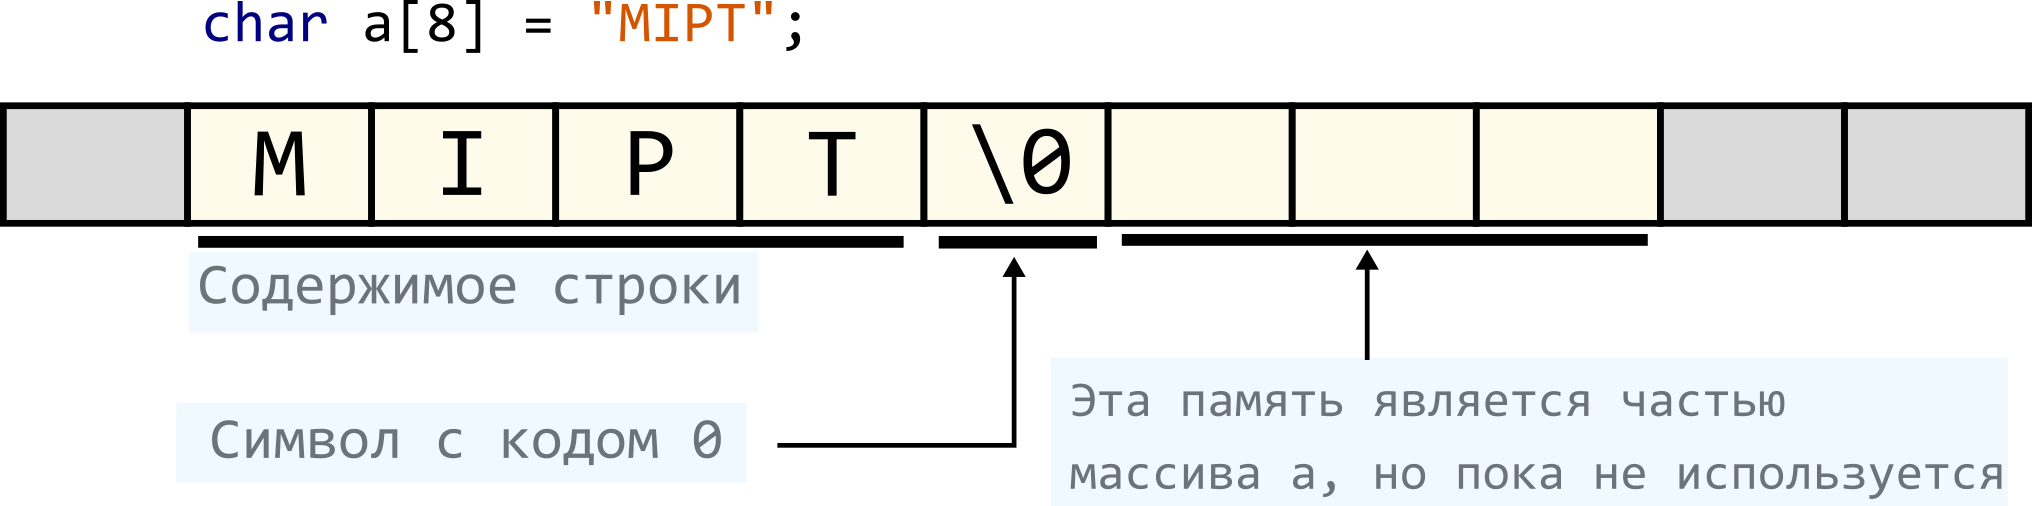
\includegraphics[scale=0.75]{../images/string_in_memory.png}
\end{center}

\subsection*{Объявление, инициализация и изменение строк}
Создавать строки можно также как и массивы, а можно и с помощью строки в двойных кавычках.
\begin{lstlisting}
char a[10] = {77, 73, 80, 84, 0};
char b[10] = {'M', 'I', 'P', 'T', '\0'};
char c[10] = "MIPT"; // Символ 0 поставится автоматически
// Использовать = со строками можно только при создании, то есть это работать не будет:
// a = "CAT";
// Изменение элементов строк работает также как и у массивов:
a[1] = 'A';
\end{lstlisting}

\subsection*{Печать строк. Спецификатор \texttt{\%s}}
Обычные массивы нельзя печатать одной командой \texttt{printf}, но специально для строк ввели модификатор \texttt{\%s}, благодаря которому можно печатать и считывать строки одной командой.
\begin{lstlisting}
char a[10] = "MIPT";
printf("%s\n", a); // Печатаем строку
\end{lstlisting}


\subsection*{Считывание строк}
Считывать строки можно с помощью \texttt{scanf} со спецификатором \texttt{\%s}. Но если вы введёте слишком большую строку,
которая не поместится в массив, то произойдёт ошибка -- выход за границы массива.
\begin{lstlisting}
char a[100];
scanf("%s", a); // Считываем строку
\end{lstlisting}

\subsection*{Безопасное считывание строк}
Чтобы указать \texttt{scanf} сколько символов можно считывать:
\begin{lstlisting}
char a[100];
scanf("%99s", a); // Безопасно считываем строку
\end{lstlisting}


\newpage
\section*{Часть 3: Строки и функции}
Строки передаются в функции также как и массивы. То есть при изменении строки внутри функции она меняется и снаружи. Но только при передаче строки не обязательно передавать её размер, так как граница строки задаётся нулевым символом. Пример функции, которая заменяет один символ в строке на другой:
\begin{lstlisting}
#include <stdio.h>
void change_letter(char str[], char from, char to) 
{
    int i = 0;
    while (str[i]) 
    {
        if (str[i] == from) 
            str[i] = to;
        i++;
    }
}

int main() 
{
    char a[100] = "Cats and dogs";
    printf("%s\n", a);
    
    change_letter(a, 'a', '#');
    printf("%s\n", a);
}
\end{lstlisting}

\subsection*{Считывание до заданного символа}
Как вы могли заметить, использование \texttt{scanf} с модификатором \texttt{\%s} считывает до первого пробельного символа. Чтобы считать всю строку (то есть до символа \texttt{'\textbackslash n'}), следует использовать модификатор \verb|%[^\n]|. \\
Пример программы, которая считывает строку и меняет пробелы на переносы строк:
\begin{lstlisting}
#include <stdio.h>
int main() 
{
    char str[100];
    scanf("%[^\n]", str);
    for (int i = 0; str[i]; i++)
    {
        if (str[i] == ' ') 
            str[i] = '\n';
    }
    printf("%s\n", str);
}
\end{lstlisting}


\newpage
\section*{Часть 4: Стандартные функции библиотеки \texttt{string.h}:}
\begin{itemize}
\item \texttt{size\_t strlen(const char str[])} - возвращает длину строки
\item \texttt{char* strcpy (char a[], const char b[]))} - копирует строку \texttt{b} в строку \texttt{a}, т.е. аналог \texttt{a = b}.
\item \texttt{char* strcat(char a[], const char b[])} - приклеивает копию строки \texttt{b} к строке \texttt{a}, т.е. аналог \texttt{a += b}.
\item \texttt{int strcmp(const char a[], const char b[])} - лексикографическое сравнение строк (возвращает \texttt{0}, если строки одинаковые, положительное, если первая строка больше, и отрицательное, если меньше)
\end{itemize}
\begin{lstlisting}
#include <stdio.h>
#include <string.h>
int main() 
{
    char a[100] = "Cat";
    char b[100] = "Dog";
	
    // Строки это массивы, поэтому их нельзя просто присваивать 
    a = b; // Это не будет работать! Нужно использовать strcpy:
    strcpy(a, b);
    
    // Конкатенация ( склейка ) строк. Можно воспринимать как +=
    a += b; // Это не будет работать! Нужно использовать strcat:
    strcat(a, b);
	
    // Строки это массивы, поэтому их нельзя просто сравнивать
    if (a == b) {...} // Это не будет работать! Нужно использовать strcmp:
    if (strcmp(a, b) == 0)) {...} 
}
\end{lstlisting}


Также могут быть полезны следующие функции из библиотеки \texttt{stdio.h}:
\begin{itemize}
\item \texttt{sprintf} - аналог \texttt{printf}, но вместо печати на экран, 'печатает' в строку.
\item \texttt{sscanf} - аналог \texttt{scanf}, но вместо считывания на экран, 'считывает' из строки.
\end{itemize}


\newpage

\section*{Часть 5: Аргументы командной строки}
Программы могут принимать аргументы. Простейший пример -- утилита \texttt{ls}. Если запустить \texttt{ls} без аргументов:
\begin{verbatim}
    ls
\end{verbatim}
то она просто напечатает содержимое текущей директории.  Если же использовать эту программу с опцией \texttt{-l}: 
\begin{verbatim}
    ls -l
\end{verbatim}
то на экран выведется подробное описание файлов и папок в текущей директории. В данном примере опция \texttt{"-l"} является аргументом командной строки. \\

В случае передачи информации программе через аргументы командной строки, информация передаётся при вызове 
программы. Чтобы передать что-либо программе через аргументы командной строки, нужно
написать это в терминале при запуске программы сразу после её запуска.

Например, если мы хотим передать программе \texttt{a.out} строку \texttt{cat}, то программу нужно вызвать так:
\begin{verbatim}
    ./a.out cat
\end{verbatim}

Если же мы хотим передать программе \texttt{a.out} число \texttt{123}, то программу нужно вызвать так:
\begin{verbatim}
    ./a.out 123
\end{verbatim}
Только нужно помнить, что аргументы командной строки всегда воспринимаются как строки и в данном случае 
число \texttt{123} передастся как строка \texttt{"123"}.

\newpage

\section*{Часть 6: Чтение из файла в строку}
Пример программу, которая подсчитывает количество слов в файле.
\begin{lstlisting}
#include <stdio.h>
#include <string.h>
int main() 
{
    // Считывание слов из файла
    FILE* infile = fopen("words.txt", "r");
    char words[500][100];
    int number_of_words = 0;
    while (fscanf(infile, "%s", words[number_of_words]) != -1) {
        number_of_words++;
    }
    fclose(infile);
}
\end{lstlisting}
\end{document}